\chapter[Simulação e Resultados]{Simulação e Resultados}

%\section{asdf}
A simulação foi realizada no Cadence usando a tecnologia 0.18 UMC. Para observar a ativação de todas as faixas de frequência fornecidas pelo circuito, foram ajustadas 3 fontes com atraso de início para ativar as entradas no integrador. Ao fazer a simulação transiente as faixas de frequência obtidas foram:

\begin{itemize}
\item 101,6Hz	 \----	991Hz
\item 1,014kHz \----	9,764kHz
\item 10,50kHz \----	93,57kHz
\end{itemize}

A potência máxima consumida é obtida quando o VFC fornece a maior frequência possível. Ao fornecer uma tensão $V_{in}$ de 2,5V e o resto do circuito com tensão de alimentação $V_{DD}$ de 1,2V a máxima potência média calculada foi de $10,03\mu$W.


\begin{figure}[htb]
	\centering
	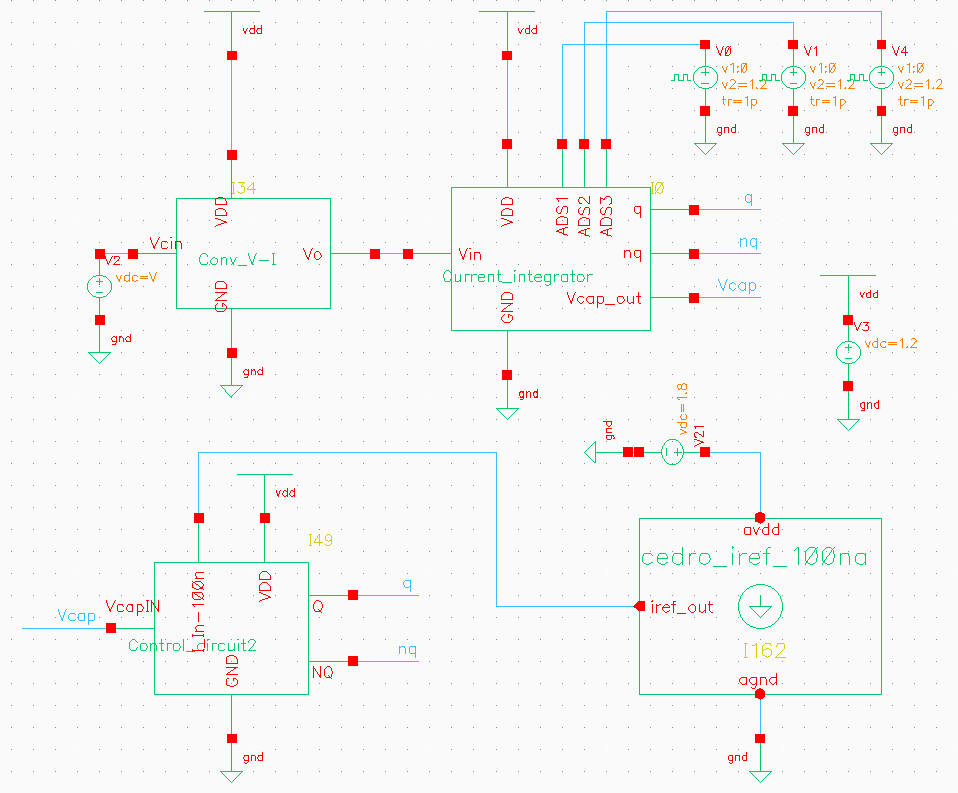
\includegraphics[width=0.9\textwidth]{figuras/imgs_jv/top.png}
	\caption{ Esquemático de topo com integração de todos os sub-circuitos do projeto }
	\label{fig16}
\end{figure}

\section{Latch SR}

\begin{figure}[htb]
	\centering
	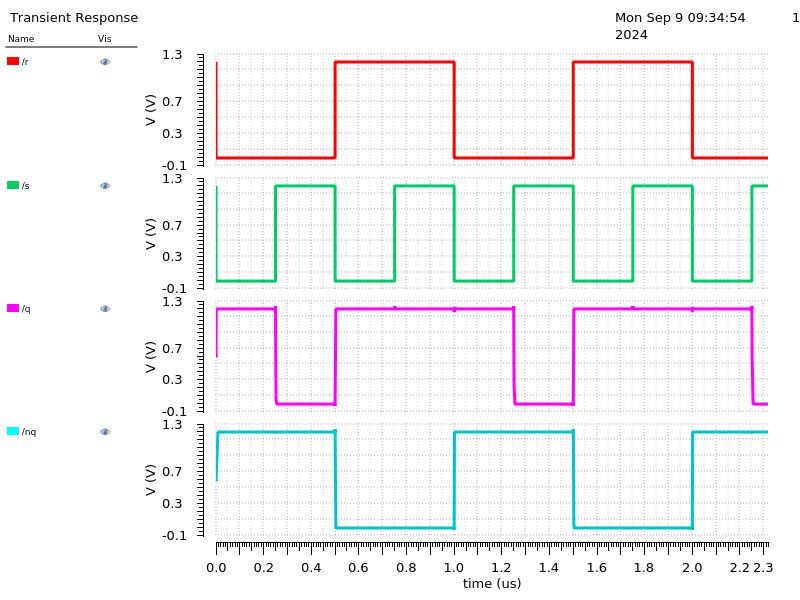
\includegraphics[width=0.9\textwidth]{figuras/imgs_jv/sim_lach.jpg}
	\caption{Simulação do Latch SR no Cadence }
	\label{fig17}
\end{figure}


\section{AmpOp}

\begin{figure}[htb]
	\centering
	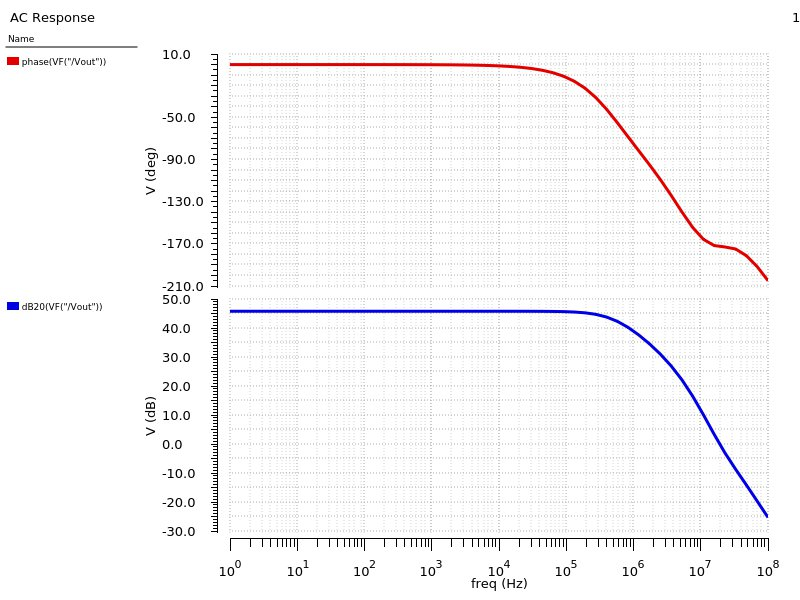
\includegraphics[width=0.9\textwidth]{figuras/imgs_jv/sim_ampop.jpg}
	\caption{ Simulação no Cadence do modelo de AmpOp usado no circuito de controle }
	\label{fig18}
\end{figure}





\section{Conversor tensão corrente}

A relação entre a tensão $V_{in}$ e a corrente de saída do VIC está na Fig. \ref{fig17}. Observa-se no gráfico que os limites da faixa de correntes mínimas e máximas são:
\begin{itemize}
\item $1,2$V	 \----	$68,2n$A
\item $2,5$V \----	$703,8n$A
\end{itemize}

As correntes espelhadas no integrador seguem o comportamento desse conversor, portanto a linearidade de ambos são iguais. Por conta disso um VIC mal feito acarretaria erros acumulados, como pouca linearidade, faixa de frequência e consumo de potência, que dificultariam o funcionamento esperado dos outros circuitos.


\begin{figure}[htb]
	\centering
	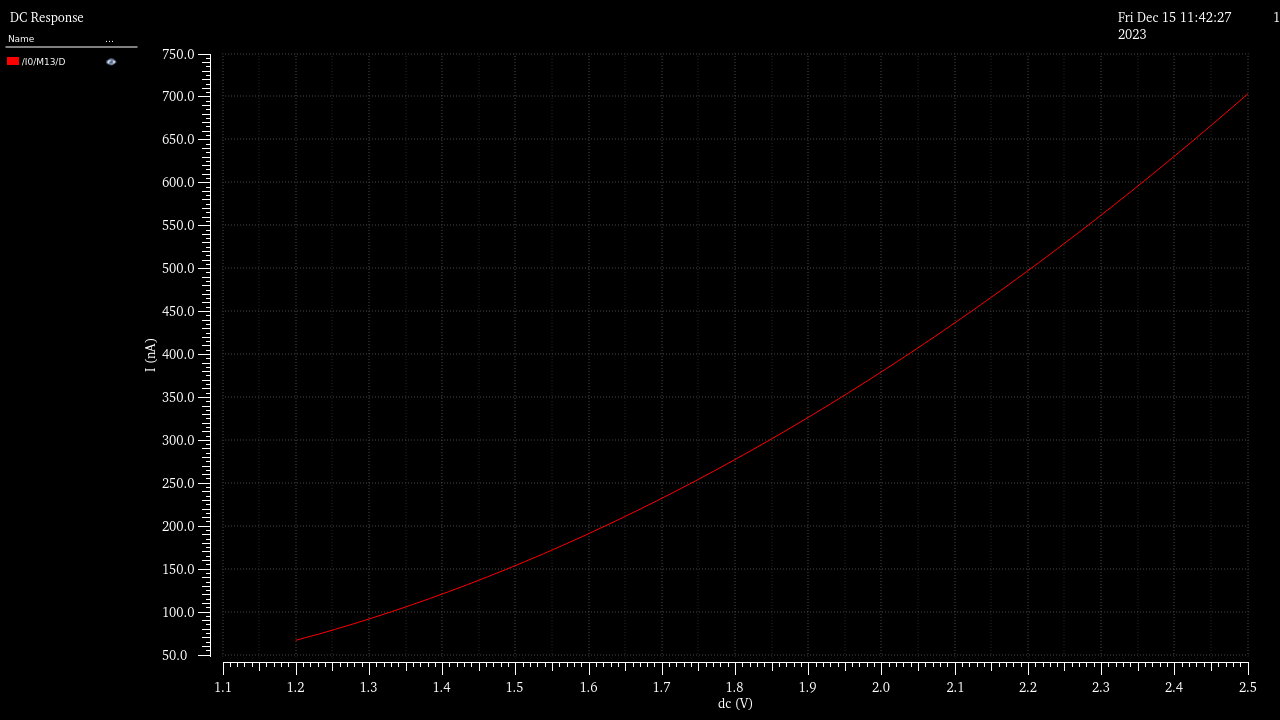
\includegraphics[width=0.9\textwidth]{figuras/sim_VIC.png}
	\caption{ Simulação da corrente de referência espelhada na Saída do VIC }
	\label{fig17}
\end{figure}

\section{Circuito de Controle}

Na Fig. \ref{fig18} está os sinais observados no circuito de controle. Nota-se o acionamento dos sinais $S$ e $R$ no Latch com a queda abrupta nos AmpOps nos sinais verde e laranja. O sinal verde é o sinal $R$ cuja é a resposta do comparador que percebe que $V_{cap}$ atingiu $V_H$, ao cair, aciona no Latch a rotina de descarga do capacitor. Inversamente ao perceber que $V_{cap}$ ficou menor que $V_L$ o sinal $S$ cai e o Latch aciona a rotina de carga.

A tensão $V_{cap}$ é observada na onda triangular em azul e a onda quadrada é o sinal em frequência do VFC e saída $Q$ do Latch.

\begin{figure}[htb]
	\centering
	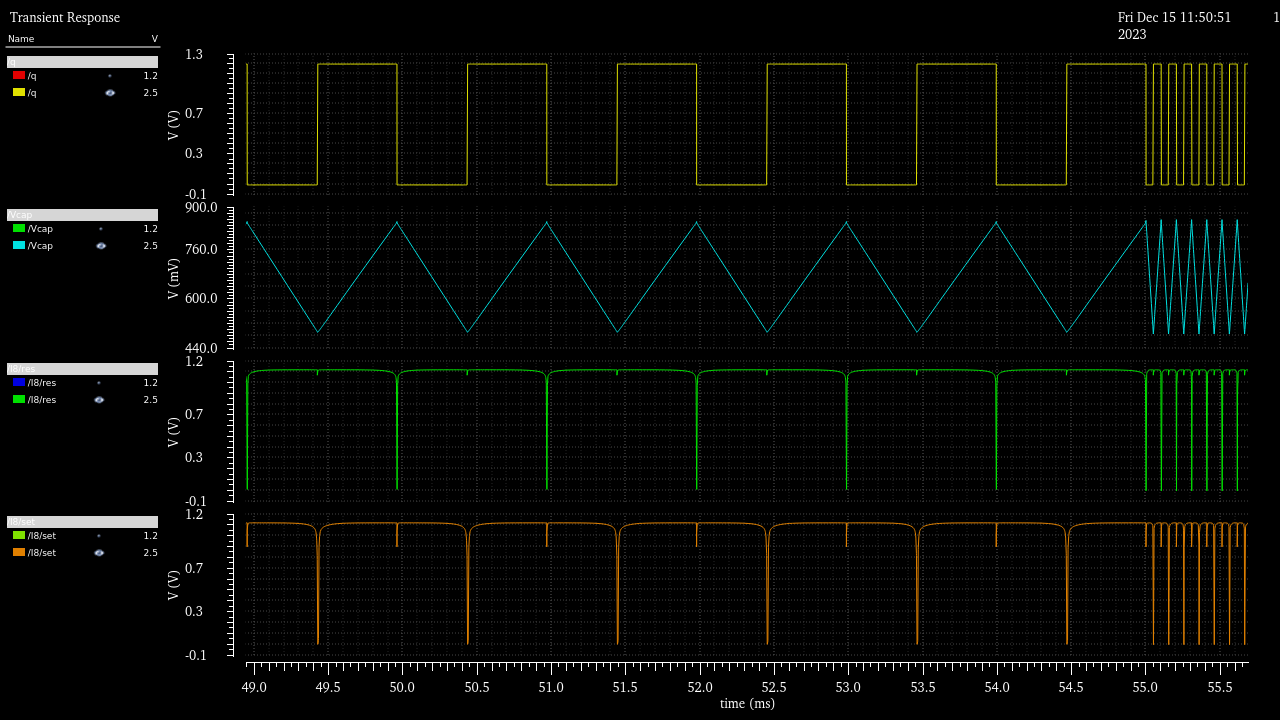
\includegraphics[width=0.9\textwidth]{figuras/sim_controle.png}
	\caption{Sinais observados no Circuito de Controle }
	\label{fig18}
\end{figure}



